\newif\ifpdf
\ifx\pdfoutput\undefined
\pdffalse % we are not running PDFLaTeX
\else
\pdfoutput=1 % we are running PDFLaTeX
\pdftrue
\fi

\documentclass[a4paper]{article}
\usepackage[swedish, english]{babel}
\usepackage[T1]{fontenc}

\ifpdf
\usepackage[pdftex]{graphicx, color}
\renewcommand{\encodingdefault}{T1}
\renewcommand{\rmdefault}{pad}
\pdfcompresslevel=9
\else
\usepackage{graphicx, color}
\fi

\usepackage{fancyhdr}
\pagestyle{fancy}

\lhead{\small{\textit{Frisk, �stersj�}}}
\chead{}
\rhead{\small{\textit{Negotiating the Musical Work}}}

\usepackage{url}

\makeatletter
\def\url@leostyle{
  \@ifundefined{selectfont}{\def\UrlFont{\sf}}{\def\UrlFont{\small\ttfamily}}}
\makeatother

\urlstyle{leo}

\title{Negotiating the Musical Work. \\An empirical study on the
inter-relation between composition, interpretation and performance}
\author{Henrik Frisk\\{\small PhD candidate}\\{\small Malm� Academy of
Music - Lund University}\\{\small henrik.frisk@mhm.lu.se} \\ 
Stefan �stersj�\\{\small PhD candidate}\\{\small Malm� Academy of
Music - Lund University}\\{\small stefan\_ostersjo@hotmail.com}}

\date{29 January 2006}

\begin{document}
\selectlanguage{english}
\maketitle

\thispagestyle{empty}

\begin{abstract}
In this paper we intend to explore the inter-relations between performer
 and composer, in the form of a theoretical study, which is intended to
 lay the ground for a new work for guitar and computer by Henrik Frisk
 for Stefan \"{O}stersj\"{o}. This project is part of our respective artistic
 research projects at the Malm\"{o} Academy of Music and is an effort to
 combine reflection, analysis, and empiricism in the framework of
 artistic research.

We find that the ontology of the mixed media work (in lack of a general
 terminology we use the term 'mixed media' in this article to refer to a
 work for instrument(s) and electronic sounds) is closely related to the
 general discussion of score-based works, but it is important to bear in
 mind that the programming of the electronics should also be regarded as
 notation in this discussion and the electronic part is itself another
 object of interpretation for the performer.

%From a hermeneutic point of view, performance interpretation of music is
% a special case \cite{levinson,davies,stecker}\nocite{krausz}. When
% elements of electronic real-time processing, sound synthesis, sound
% file playback or be it any other means of producing electronic sounds,
% are part of the work, yet another level of complexity is added to the
% issue of interpretation. This is closely related to the notion of
% authenticity, which is already a powerful factor in the performance of
% score-based works. How is this issue to be aproached in mixed media
% works? If the programming of the electronic part is to be regarded as a
% special case of notation, how is this notation 'transcribed' and
% communicated to the performer?
% 
%A close collaboration between a living composer and a performer, allows
%for discussions on the rendering of a mixed media work. We find that
%this process could be described as a negotiation towards a version of
%the work \cite{kivy} and that this can serve as a model for
%understanding similar processes even prior to the existence of any
%notated material. This article aims at a closer understanding of the
%significance of these negotiations, specifically their meaning in
%relation to the two modes of musical representation; the notation and
%the sonic trace left by the computer part. Further, we aim at creating a
%broader platform for reflection on and analysis of our respective
%artistic practices.
%
We approach this complex area empirically by analyzing selections of the
 video documentation of �stersj�'s collaboration with composer Love
 Mangs, as well as versions of a certain passage in a piece for harp and
 computer by Henrik Frisk. Love Mangs' ``Viken'' is a work for guitar,
 banjo, e-bow and real time processing in Max/MSP. In the video material
 we find striking examples of how the traditional roles of "composer"
 and "performer" are exchanged, indicative of the difficulty to
 establish fixity in the definition of these seemingly discrete artistic
 fields. By using Molino's and Nattiez' terminology for
 a semiological analysis of music we attempt at describing the interplay
 in terms of poietic and esthesic processes, \cite{nattiez}
 \cite{molino} and with semiotic terminology in general.

\end{abstract}


\section{Introduction}
This article discusses the musical work prior to its ultimate notation
and prior to its performance; we discuss the musical work in the Western
art music tradition, in which musical notation has an ontologically
crucial function. The article deals exclusively with music for solo
instrument and live electronics. Our purpose is to acquire a deeper
understanding for the underlying processes in the communication between
the composer and the performer and their respective roles. Obviously one
of the fundamental conditions for a study such as this is that the
performer and the composer are both alive, and that the performer has a
genuine interest in performing the work in question. By better
understanding the musical interaction between the two parties involved
in the creation of the work, we also hope to better understand the
necessary conditions for a successful interaction between the performer
and the electronics.

As for works, we find useful a distinction between art works made by
Nelson Goodman. Works depending on notation (like literature,
choreography, music specified in scores) are allographic and works where
the artist - basically - produces an object are autographic. Autographic
works can be falsified: In fact, even the most precise duplication
always results in a false copy. Allographic works can have many
instances, deriving their mutual identity from the notation. A musical
work, in the cultural context of the Western art music tradition, is
commonly regarded as the result of a process in two distinct phases; one
constructive and one reproductive. The composer produces a score (an
allographic musical work) which in turn is handed over to a performer
who makes an interpretation of the notation and reproduces it as
specified in the score, hopefully quite faithfully to the composer's
intentions. The notation constitutes the primary source of information.
Since not only the problem we are facing - mapping the communication
between two parties on the interpretation of a yet not notated piece of
music and its electro acoustic part - but also the entire field of mixed
media musical works is severely lacking of an accepted and widespread
terminology we find that it is of great importance to use a method whose
terminology is defined. Musical semiology has been constructed with the
intention to provide tools for analytical understanding of the musical
work in its entirety, and not only in terms of analysing formal
structures or details in the construction, but also the socio-cultural
context. Attempting to move to a lower level of organization than that
of musical notation may help to further clarify the issue in relation to
a wider sphere of knowledge.

\subsection{Music and notation}
Although the degree of mystical fascination for abstract ways of
constructing music has varied, the history of Western art music displays
a bit-by-bit increasing focus on notation. This has resulted in an
expanding interpretative and analytical practice, which takes the
notation and not the sound as its point of departure.

Following Trevor Wishart, we find that the development of notation has
given us notions such as that of the composer and the musical work. The
core of the argument in Wishart's 'On Sonic Art' \cite{wis96} is the
assumption that notation not only reflects, but actually even creates,
the priorities that are crucial in the system, and those priorities are,
in traditional notation, the categories of pitch and duration. Wishart
finds the reason for this in the inability of musical notation to
describe and quantify e.g. timbral elements of musical
sound.\footnote[1]{It can be questioned if this is the right
conclusion. In the time of Couperin or Haydn, much of the expression in
music was left to performance practice. The fact that timbre or
articulation cannot be rationally organized doesn't give for granted
that it is subordinate.} And further, as the musical organisation of a
score-based work relies on constructions that take the parameters that
are possible to notate and permutate etc. as point of departure, this
gives us a split in conception between primary and secondary aspects of
musical parameters. What follows from this is a redirection of the
perception of music towards aspects of sound that can be analysed and
rationalised from the score. In other words, and following the line of
thought in 'On Sonic Art', the center of Western art music has often
been the score and its text-based interpretations. It might be fruitful
for the discussion in this paper to consider one aspect of Wishart's
argument: The split of 'the musician' into two agents. This split calls
for an extended discussion of what composer and performer provide to the
creative process.

\subsection{The two agents} \label{twoagents}
The split between composer and performer should not be regarded as a
negative feature in Western art music; it is a necessary specialisation
in the development of a tradition that has been creative. Needless to
say, notation is an asset in many ways, giving way for experiments that
would not be obtainable by other means. We wish to consider what this
split implies for the creative process of producing a musical work. Like
Paul Ricoeur's understanding in the case of literary texts,
\textcolor{red}{we find that the composer is disengaged from the
musical text in the act of writing}. We believe that the construction of
a score-based work consists of dialectic interplay between creation and
interpretation, in which the composer, at times, has to approach his own
notation by means of interpretation, \textcolor{red}{during the act of writing.} In other
words, notation does not divide composer and performer into one
interpreter and one originator. Interpretation is a part of both
creative acts.

From a hermeneutic point of view, performance interpretation of music is 
a special case \cite{levinson,davies,stecker}\nocite{krausz}.
\begin{quote}
If performances and critical interpretations are both representations of
works, they are so in quite different senses. If we ignore these
differences, we can easily be misled to make invalid
inferences. Performances are necessarily constructive; that is, they
necessarily add features that the work leaves vague or
undetermined.\cite{stecker} 
\end{quote}

But not only in cases in which the notation is in some respect unclear
or vague is there a call for constructive elements in
interpretation. Construction is really at the heart of the matter in
performance interpretation. And further, when elements of electronic real-time
processing, sound synthesis, sound file playback or be it any other
means of producing electronic sounds, are part of the work, yet
another level of complexity is added to the issue of
interpretation. This is closely related to the notion of authenticity,
which is already a powerful factor in the performance of score-based
works. How is this issue to be approached in mixed media works? If the
programming of the electronic part is to be regarded as a special case
of notation, how is this notation 'transcribed' and communicated to
the performer?

It has been suggested by several writers that performances should be
regarded as works in their own right. From this point of departure,
Peter Kivy \cite{kivy} distinguishes between four kinds of authenticity
in performance, most importantly; 'Authenticity as Intention' (that is,
authenticity as faithfulness to the composer's performance intentions)
and a fundamentally opposed notion of authenticity, which he simply
names 'The Other Authenticity'. Kivy's intention is to
bring out an opposition between these two authenticities: On the one
hand, the obligation to conform with the composer's intention and, on
the other hand, the creative originality that should result in a work in
its own right. But, unlike Kivy, we suggest (as has been done by Stefan
\"{O}stersj\"{o} and Cecilia Hultberg \cite{ost05}) that the opposite may also
be claimed: The tension between the two imperatives on the performer
makes up a creative field in which truly original instances of works
come out. The different forms of authenticity turn out to be the
definition of a creative field of tension in which the composer and the
performer negotiate and interact towards a version of a work.

\subsection{Mixed media}
If we can see Western art music as a practice in which the labor is
split up in two agents, in Mixed Media works we can observe a blurring
of the line of division between the composer and the musician that holds
significance for the discussion above on authenticity, but also for the
analysis below. But before we go further into that issue we need to
clarify what we mean by the term 'mixed media'.

In our definiton mixed media music includes, but is not limited to,
music in which sounds produced on acoustical instruments are mixed with
sounds from electronic sources or electronically processed versions of
the acoustic sounds played back on loudspeakers. One medium of sound
production (acoustical instruments) is mixed with another
(loudspeakers). One of the issues with mixing these two mediums of sound
production is the different prerequisites that they have.

\subsubsection{The technology of notation and of the studio}

While considering the specific nature of mixed works it might be
fruitful to take into account the similarities and dissimilarities
between the technology of notation and the technology of digital or
analogue electro acoustic techniques. There is a striking parallel in
the fixity of a musical work resulting from notation and that derived
from pre-prepared electronic real time processing. The notation in the
computer program makes these works more like allographic than
autographic works. The most important difference is of course that the
languages in which computer programs are written are not intended for
interpretation, neither by the machine nor by a human being. The
object of interpretation for the performer is not the 'notation'
but the sounding result of the electronic treatment. In other words,
if we regard the pre-prepared structure as another kind of notation
the possibility of interaction between the performer and the resulting
electro-acoustic music becomes of great interest.

Does this make improvisation on pre-prepared materials more like the
performance of notated works in general? I believe this is often the
case. Of course there is a different situation when there is a
computer part, which generates an unpredictable and radically
different sounding result to what is being produced by the
performer. But generally the similarity should be noted, improvisation
with a fixed sequence of timbral treatments on an improvisation can be
very similar indeed to performative interpretation of allographic
works.  Does this mean that the computer files should be regarded as
an allographic work?

The dependence on technologically fixed sounds and real time treatment
of acoustic sounds, make mixed works into a distinct ontological
kind. Stephen Davies (2001:34-36) distinguishes works that are for
live performance from those that are for studio performance. In the
former kind we find e.g. allographic works for acoustic instruments,
in the latter we find rock music using sophisticated technical devices
for treating and layering sounds. Works for studio performance take
aspects of instrumental playing into account while still putting focus
on the ultimate result of the studio productions as issued on a
commercial recording intended for playback on appropriate machines. I
would like to suggest that mixed works are to be regarded as works for
studio performance with the exception that they are by practice
normally brought to live performances aiming at a real time
performance of the entirety of information to be found in a studio
recording of the work.

What then with the performer's autographic work, the performative
interpretation, are there any differences to be found in the
conditions in a performance of a mixed work? I believe this is the
case. The perhaps most important aspect is not to found in the
different technical solutions of synchronisation but in the way the
sound is projected to the listener. Many composers in this field take
a great interest in the possibilities of surround projection of sounds
and the mixture of acoustic and electronic sounds into an undefined
area where new timbral possibilities emanate from the combination of
the two sound worlds. This makes the diffusion at the mixing desk an
important aspect of the performance. In other words, a typical solo
performance of a work of this kind is to be regarded as a duo
performed together with a sound engineer, often being the composer. It
has been suggested by Simon Emmerson that ideally the electronic sound
should be projected from stereo loudspeakers close to the performer,
playing without amplification, so that the performer is in control of
the totality of the sounding work and the listener is the also able to
tell which is the source for the different timbral layers of the
music. I doubt that this is a solution of general validity. It should
rather be acknowledged that the sound engineer and the instrumentalist
should prepare an interpretation together as a duo, leaving the
resulting sound in the performance a subject of negotiation between
the two.

\section{Musical semiology}
\begin{quotation}
\begin{textit}
{Thus the myth and the musical work are like conductors of an orchestra,
 whose audience becomes the silent performers. If it is now asked where
 the real center of the work is to be found, the answer is that this is
 impossible to determine.}
\end{textit}
\cite{lest69}
\end{quotation}
As difficult as it may be to define the elusive 'center' of a work of
music, as a composer or performer we need to ceaselessly strive, at
every moment along the creative process, to aim at this ontological
focus point, well aware that at the same time we define it the center
will have moved. When reading the quote above we need however remember
that L\'{e}vi-Strauss had a very rigid understanding of the artwork. The
organising principle of tonality is a structure that according to him,
by physical fact cannot be disputed and, when ignored, deprives music of
the first articulation in a semiological analysis just as non-figurative
painting does in the case of visual arts.The line of thought expressed
by L\'{e}vi-Strauss in his discussion of the artwork has been vividly
debated and is in itself an indication of the dangers of an unrelenting
belief in methodology (see \cite{eco71,der82}).

Jean-Jacques Nattiez offers an excellent review of the history of
musical semiology in `Reflections on the development of semiology of
music' in which he gives an historic perspective on semiological
approaches to fundamental issues such as; ``What is the nature of
musical signification?''. Nattiez distinguishes between intrinsic and
extrinsic significations within musical semantics, finding the former to
be to a large extent founded on the work of Nicolas Ruwet and the notion
of music as a language that signifies itself \cite[pp. 30]{nat89}. Jean
Molino summarizes Susanne Langer's idea of music as the `unconsummated
symbol' and captures the essence of the problem: ``On the one hand, the
unchallengeable presence of evocation; on the other, the impossibility
of exploiting it.'' \cite[pp. 126-7]{molino} Umberto Eco points to the
problems with connecting the investigation of a sign with the object to
which it refers. It is impossible to attribute logical statements such
as 'true' or 'false' to the semiological investigation of music and for
Eco these are pre- or postsemiotic problems; ``The signs are of interest
to semiotics as social powers'' and further ``Any attempt to establish
the referrent of a sign will force us to define this referrent with the
terminology of an abstract entity.'' This is what Eco calls the
``cultural convention''. \cite[pp. 61-6]{eco71}

Defining a cultural context as the referrant resolves some issues in the
analysis of performed music as the listener or concert-goer can be
defined as belonging to a cultural entity - a cultural entity that may
be used as the code to decipher the message, which in this case is the
acoustical trace left by the performed music. However, in our study we
are looking at a not yet existing work - a work in progress. Following
the same model we might try to understand the symbolic system in
relation to a subculture created by the agents involved. Both composer
and performer are working within the frame of their own cultural context
which defines their respective understandings of the evolving work. The
subculture is the result of the interaction between these two
contexts. The musical work becomes the sign or the message, the agents
the signifiers and the subculture the signified or the code. Apart from
the fact that this model inevitably becomes a very \textcolor{red}{rough generalization
of reality}, it is also highly dependent on the definition of the
cultural context, which in the case of composer-performer interaction
prior to the existence of a work becomes a very complex task. The model
suggested by Molino for analysis of music appears to be a more flexible
method for our study.

\subsection{The three dimensions} \label{threedim}
Molino reminds us that the hypothesis that there is a 'single,
well-defined item of information to be transmitted, all the rest being
simply noise' is 'dangerously inaccurate and misleading as soon as we
move from the artificial communication of information to a concrete act
of human communication as a total social fact.' \cite{molino} Music,
according to him, is a product and not a transmission. Marcel Duchamp
describes the work of art in a similar fashion; as two poles with the
artist on the one side and the viewer on the other. The intention of the
artist holds no significance to the work's interpretation. Molino
further refers to Paul Val\'{e}ry, to point out that 'there is no
guarantee of a direct correspondance between the effect produced by a
work of art and the intentions of its creator'. Hence Molino suggests a
model for symbolic analysis on three levels; 'the poietic, the esthesic
and the 'neutral' analysis of the object'. Three modes all representing
the same work of art. The poietic level is the constructive phase, the
esthesic is the interpretative phase and the neutral is the trace left
by the poietic (or esthesic) process. The analysis at the different
levels does not necessarily have to lead to the same conclusions or
results, thus connecting the method of analysis to the statements above
by Duchamps and Val\'{e}ry.

What kind of significance does the idea of a tripartite analysis hold
for our study?  \textcolor{red}{That it provide the tools for analysing
and understanding the inter-relation between composer and performer
certainly is the point of view of one of the most important proponents
of musical semiology, Jean-Jaques Nattiez:}
\begin{quotation}
...recognizing, elaborating, and articulating the three relatively
autonomous levels (poietic, neutral and esthesic) facilitates knowledge
of all processes unleashed by the musical work, from the moment of the
work's conception, passing through its 'writing down', to its
performance. \cite{nattiez}
\end{quotation}
Nattiez discusses the important issue of where the poietic process ends
and the esthesic begins in score-based music \cite{nattiez}. In essence
a different terminology for the same ontological discussion of the
musical work as above: What is the musical work, is it the graphic sign
alone or is the musical work incomplete before it is realised as sound
in performance? Nattiez finds that the greatest difference, between the
score and the acoustic trace left by a performance, is that while the
score is 'an invariable physical reality' there are just as many
acoustic realisations as there are performances. The performance
interpretation is the borderline between the esthesic and the poietic
field. At this point Nattiez leaves the discussion open, and turns his
attention to critical interpretation. The difference between
performative and critical interpretation is beyond the scope of the
present paper but has been thoroughly discussed e.g. by Jerrold Levinson
\cite{levinson}. Nattiez finds that critical interpretation comes into
play in between the score and its performance and takes this as an
argument for semiological analysis to approach the score-based musical
work in the same way. According to this line of thought, he finds that
the graphic sign precedes interpretation. For this reason he suggests
that neutral level analysis should be devoted only to the graphic
sign. We believe that this is an oversimplification of the actual
processes taking place. As we suggest in (\ref{twoagents}) the process
of writing a musical work is not a unidirectional poietic process. The
act of writing should be understood as an interaction between esthesic
and poietic processes, overlapping and interacting in the creative
process in a way that makes it impossible at a detailed level neither to
define the end of the poietic process nor the beginning of the esthesic.

According to Nattiez, in a semiological analysis of a musical work it is
necessary to approach any kind of music by ways of either a descriptive
notation (transcription) or a prescriptive notation by a
composer. Semiological analysis cannot be carried through without access
to notation. This does not make up a problem in the case of our own
study, as we are studying the interaction between the two agents
inovolved and not the piece in itself, but for 'mixed music' in general
this of course creates a methodological problem. Making graphic scores
for electroacoustic works has been tried by scholars and composers ever
since the early days of electronic music, there is no doubt that there
has been little of great success in this pursuit. However, Nattiez is in
fact himself very optimistic: 'On the neutral level, it would be easy
enough to identify and describe the sound-objects that make up these
works, to describe the laws governing their succession and their
integration into various syntactic arrangements, on various levels.'
\cite[p.101]{nattiez}

In his discussion of electroacoustic music and Schaeffer's 'Trait\'{e}
des objets musicaux' Nattiez suggests that the kind of 'concentrated
hearing' that Schaeffer discusses should be understood as part of the
poietic process. \cite[p.95]{nattiez} Following this example of flexibility,
we will choose to use the terminology in a way that leaves scope for
processes that on a global level are to be regarded as poietic, as being
divided in both esthesic and poietic sub-levels while studied in closer
detail.

\textcolor{red}{Borde vi ha en mer utf�rlig diskussion om den eventuella
neutrala analysniv�n. JAg har en k�nsla av att vi springer f�rbi den litegrand...}
\section{Empirical study} \label{empirical}
\subsection{Harp piece} \label{harp}
\begin{figure}[!ht]
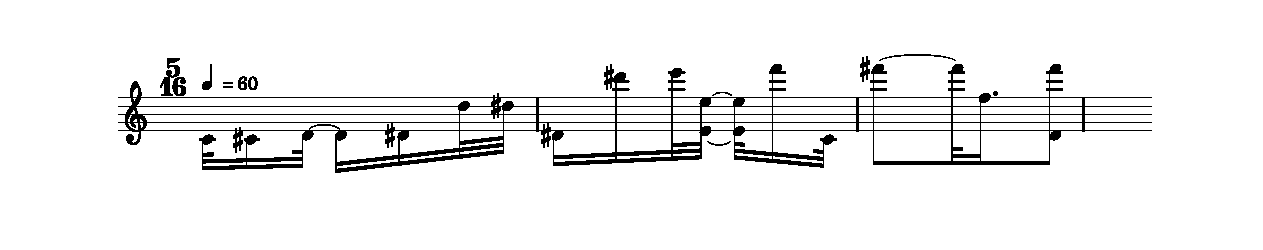
\includegraphics[width=1.0\columnwidth]{img/score/eps/harpVersion1}
\caption{First transcription of the idea into notation.}
\label{harpex1}
\end{figure}

The work discussed here is a work in progress. It was commissioned by the
Mexican harpist Mercedes Gomez in 2004 for harp and computer and the
piece is scheduled for premiere in September 2006. The melodic material
used for the piece consists of a small six note fragment that is
transposed and repeated creating a tone row of potentially infinite
length. This material is very chromatic and for that reason it isn't
idiomatic for the harp. Consequently the process of adapting this music
for the harp will inevitably involve constructive interpretation,
performed by the composer on his own musical idea. Expressed differently
we could say that the composer is working in the esthesic domain on the
trace left by the poietic act of generating the first molecules of the
evolving piece.

\begin{figure}[!ht]
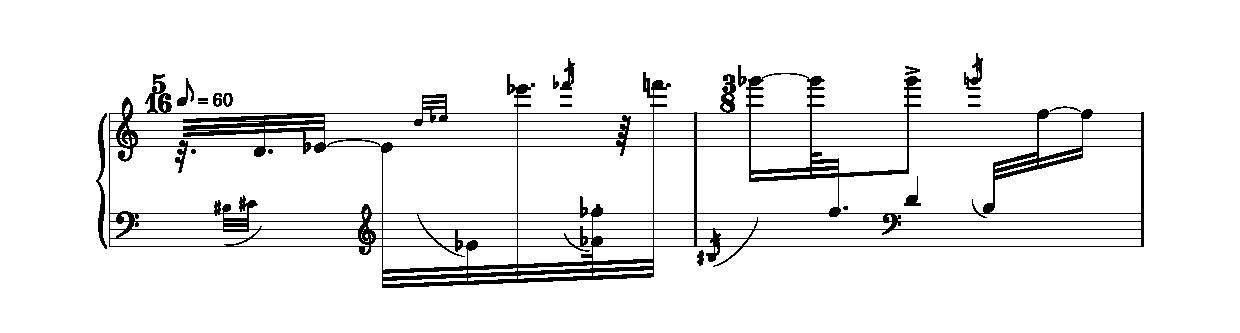
\includegraphics[width=1.0\columnwidth]{img/score/eps/harpVersion2}
\caption{First transcription for the harp.}
\label{harpex2}
\end{figure}

The following is a discussion on four notations of the same two bars of
music. The first (Figure \ref{harpex1}) is the original idea transcribed
as closely as is meaningful into the atomized rhythmic structure of
western notation. The basic musical idea at this spot is to have the
same variation of the tone row in three individual lines, separated by
octaves, each one following its own unique and entirely notated
rallentando.

\begin{figure}[!ht]
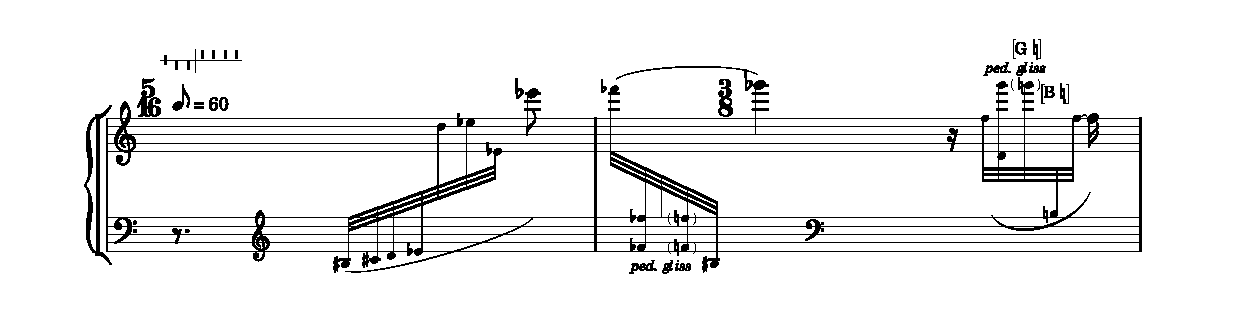
\includegraphics[width=1.0\columnwidth]{img/score/eps/harpVersion3}
\caption{A transcription rhythmically less complex.}
\label{harpex3}
\end{figure}

\begin{figure}[!ht]
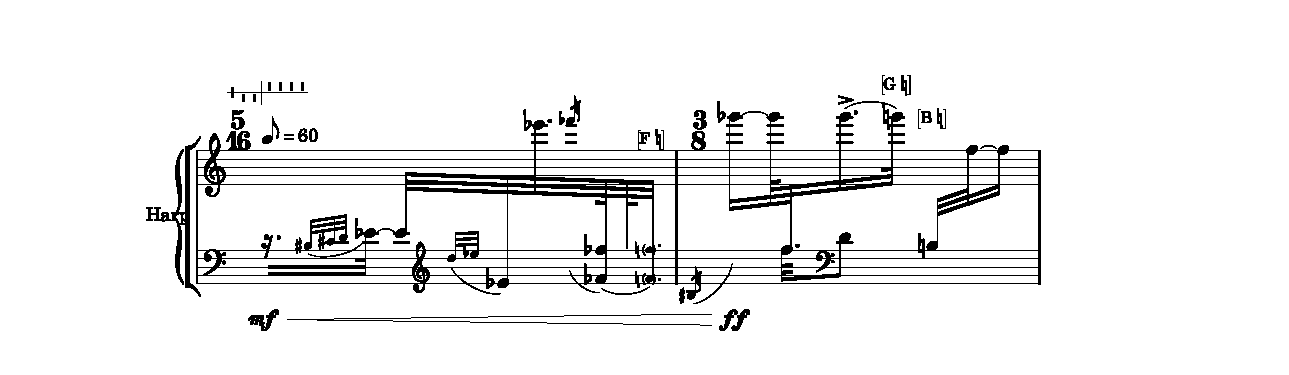
\includegraphics[width=1.0\columnwidth]{img/score/eps/harpVersion4}
\caption{A final version. More idiomatic than the example in Figure
\ref{harpex1}, but closer to the original idea than Figure
\ref{harpex3}} \label{harpex4}
\end{figure}

In the second example (Figure \ref{harpex2}) we find the first attempt
at transcribing the musical idea for the harp. Pedal changes are not
notated. At the indicated tempo, these two bars are still virtually
unplayable on the harp. The F flat to F natural pedal change at the end
of the first bar is a technical problem as is the G flat to G natural on
the second eighth note of the second bar. After working on this passage
with the harpist a version in the lines of Figure \ref{harpex3} was
suggested.

The third example (Figure \ref{harpex3}) is rhythmically less
complex. With a few written indications the effect of the slowing down
of the music could be approximated. The pedal changes are resolved by
means of pedal glisses. However the independent lines cannot be traced
in this image and the rallentando has to be described in text.

In the final example some of the rhythms has been simplified by use of
grace notes. As in the previous example some of the pedal changes have
been changed into pedal glissandos thus making the idiomatics of the
instrument part of the lines.

Considering the esthesic processes in the evolving notation of this
passage in the light of the discussion in Section \ref{twoagents}, it
vmight be worthwhile to consider the significance of Henrik's conceptual
vision of the work and how the negotiations between this musical matter
(immaterial as it may seem) and the idiomatic constraints of the harp
lead up to a version of the work in musical notation. And further, how
the presence of the performer in this discussion provides new impulses
for the piece. The original vision is the trace that constitutes the
source for the interpretative, i.e. esthesic, actions leading to the
different notations.
%
%In this context 'the work' is
%the conceptual vision, in whichever way it comes to the
%composer. However, as the following analysis shows, it makes little
%sense to isolate one certain point in this process claiming that it
%alone should make up 'the work'. Rather, it seems fair to assume that
%the musical work is the product of a complex chain of poietic and
%esthesic processes working together in an infinite loop.
%
%
%A musical work is the product of
%a complex chain of poietic and esthesic processes, which starts out with
%the conceptual vision, in whichever way it comes to a
%composer. 
%
%It seems
%to us that it makes no sense to isolate one certain point in this
%process claiming that it alone should make up 'the work'.
%
%Referring to the discussion above, the transformation that these two
%bars of music goes through would imply that the composition is neither
%the acoustic trace left by the performance nor is it the score. It is
%the conceptual idea, the vision, of the work as it is envisaged by the
%composer. Everything else, including the notation of the music, are
%creative interpretations of this first and original notion of the work.


\subsection{Viken}
\subsubsection{Introduction}
Love Mangs' Viken for guitar, banjo, e-bow and electronics (2004-05) was
commissioned for Stefan \"{O}ster\-sj\"{o} by the Swedish Arts Grants
Committee. The project had several explicit intentions, apart from the
mere production of a work for guitar and electronics. One was to use
real time processing as the main source of electronic sound, the other
was to explore the boundaries between composing and performing; between
the performance interpretation of a work and how different kinds of
fixity can be established in a work. This should be taken into account
when studying the video documentation of this process. It would be a
mistake to regard the material as documentation of a typical
collaboration between a composer and a performer, as both Love and
Stefan were well aware of the underlying intention to explore the
possibilities for improvisation and other interactive ways for composer
and performer to approach the process of creating a score-based work
with electronics. While studying the video it is also of importance to
remember that both parties involved are aware of their process being
documented. However, the session is taking place less than two months
prior to the scheduled premiere which implies that both parties are
strongly focused on the task of getting the piece together.

The transcription has played an important methodological role in our
analysis and can be found at
{\url{http://www.henrikfrisk.com/documents/vikenTranscript.pdf}}\newline and all
references in this text to the video refers to sections of the
transcription. The video clip is edited; sections with little or no
action are simply removed but the order of events are not altered. A
compressed version (QuickTime movie) of the edited video can be found at
{\url{http://www.henrikfrisk.com/documents/vikenMovie.mov}}. For
reference, an un\-edited version of the same passage can be found at
{\url{http://www.henrikfrisk.com/documents/vikenMovie-noEdit.mov}}. The
video was recorded during a session in the composer's studio on
September 17 2005.

\begin{figure}[!ht]
\begin{center}
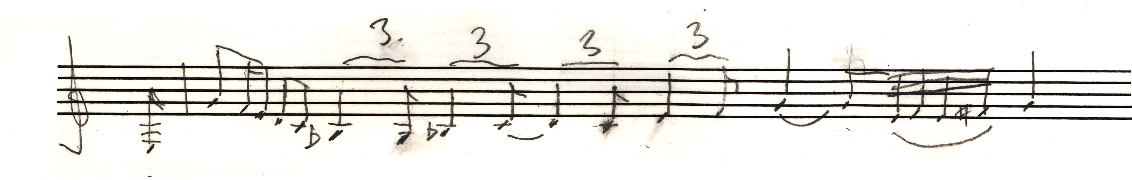
\includegraphics[width=1.0\columnwidth]{img/viken} 
\caption{Love Mangs first notation of the melody derived from the sound file.}
\label{vikentrans}
\end{center}
\end{figure}

\subsubsection{Material worked out prior to the documented session.}

It is of importance to the analysis of the communication processes in
the video to understand the material that Love and Stefan had at the
outset of the session. Love had derived a melody from a filtered
electronic sound clip, which originally wasn't intended for
\emph{Viken}. As the process of composing \emph{Viken} evolved he wanted
to include the sound file as well as the melodic material derived from
it in the work. We have already pointed out that any kind of notation
will inevitably be a reduction of the material that is the object for
transcription. Already when Love decided to make a transcription of the
sound clip he subjectively chose elements to emphasize and elements to
exclude; he is performing an act of interpretation of his own
material. He is working in the esthesic domain on the trace left by a
work performed in the poietic domain.

What is interesting with the way Love has carried out the transcription
is that he doesn't even try to establish a connection between the sound
clip and its expressive qualities in the notation. Instead he has
extracted an ordered set of discrete pitches, establishing a clear
tonality, leaving open a wide gap of possible interpretations between
the source and its representation (see figure \ref{vikentrans}). We can
say that he re-constructed a musical motif independent from its
source. In the context of his working on \emph{Viken}, what he heard in
the sound clip was the melody. An action performed in the poietic domain
as a result of working with the material in the esthesic domain but with
'knowledge of the poietics of the work' as Nattiez would put it, the
work in this case, not being the context of the sound clip but the
poietics of \emph{Viken}.

\subsubsection{Analysis of the video.} \label{thevideo}

\begin{figure}[!hbp]
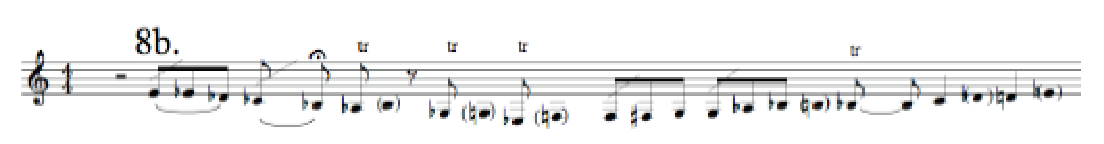
\includegraphics[width=1.0\columnwidth]{img/score/viken8b}
\caption{Material 8B from the final score of Viken.}
\label{viken8}
\end{figure}

The agreed purpose of the session documented in the video, was to work
out variations on the melody transcribed by Love. Love's intention was
to use this melodic material in the piece.

In the first scene Stefan has just played an improvisation on the melody
and on Love's suggestion he is notating the new variation (see
figure \ref{viken8}). Stefan is
active in the poietic domain, constructing new material for the
piece. He turns to Love for feedback, but at this point Love seems
remarkably indifferent. This is illustrated by the arrow going from the
\emph{new variation} box in the poietic field on Stefan's side of the
graph pointing down towards Love's side in figure \ref{graph}.  There is a lack of
communication between Love and Stefan (illustrated by the dotted arrow
going upwards from the \emph{restless, passive} box) as Love does not
respond to Stefan's invitation to discuss the new variation. Love seems
to have accepted the new material as it was played initially and instead
takes the initiative (illustrated by the initiative axis going from
Stefan's side to Love's), adopting an interpretative approach on Stefan's
variation. Love is now active in the esthesic field, suggesting to
Stefan the addition of a fermata in the variation (line 24) represented
by the \emph{fermata} box in the graph. Now there is apparent noise in
the communication (represented by the dotted arrow going from the
\emph{fermata} box to the \emph{new variation} box): Love seems unclear
of where in the notation the fermata should be. This is in turn
misunderstood by Stefan (line 59) to mean several fermatas (dotted arrow
from the \emph{several} box to the \emph{fermata} box). Eventually Love
points out the right spot and for the first time a clear communication
takes place, illustrated by the two arrows in the graph going in both
directions (line 68 in the transcription). In this segment both Love and
Stefan are acting in the esthesic domain, Love in his interpretation of
Stefan's notation and Stefan attempting to try out Love's
suggestion. Stefan's initial misunderstanding of the fermatas seems to lead to
the next initiative taken by Stefan and is illustrated by the initiative
axis going from Love to Stefan at 75. Again in the esthesic field, Stefan
suggests that long fermatas could be added to the last notes of the
phrase. At first Love doesn't get the idea at all (line 78, dotted arrow
going from the \emph{long fermatas} box to the \emph{what?} box) but eventually
approves of the suggestion (line 85, solid arrow going in the same directions).

This is followed by what seems to be an attempt on Love's part to enter
the creative discussion or to reclaim the artistic initiative. The
response from Stefan is not related to what Love says (the dotted arrow
going from the \emph{4th string} box over to Stefan's side in the graph
at line 94). The passage ends with Stefan playing the whole phrase again
giving Love a look at the end (\emph{glance} box at line 111) without
getting a noticeable response (dashed left bound arrow). It is obvious
that the communication in both directions is very noisy - this passage
is filled with unanswered questions and misunderstandings.

In the next clip Stefan is writing down the variation in more detail,
inserting Love's idea of the fermata as a normative inscription (line
119). In that sense the initiative is on Love's side, in spite of the
fact that Stefan is the physically active part with the writing. At this
point Stefan is not artistically involved, basically just making a note
of Love's interpretative idea. Love then develops his idea of the
fermatas and their significance in this passage, still active in the
esthesic domain. The way we analyze this follows a model in which the
difference between creative actions in the esthesic and poietic domains
is a difference in what class of material the creative act refers
to. Nattiez defines these as the psycho-sociology of creation and
psycho-sociology of perception respectively. Love's discussion of the
fermata emanates from his perception of Stefan's improvised new
variation at the very beginning of the video clip and is therefore to be
regarded as an esthesic process.

\begin{figure}[!hbp]
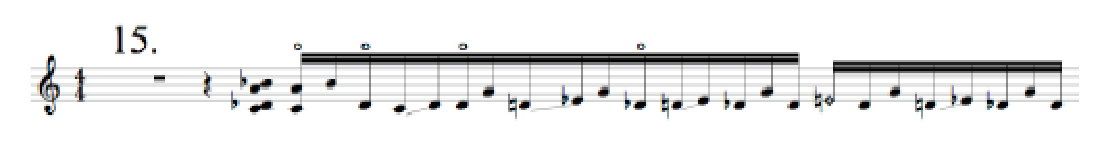
\includegraphics[width=1.0\columnwidth]{img/score/viken15}
\caption{Material 15 from the final score for Viken.}
\label{viken15}
\end{figure}

The idea of inserting several fermatas, which in the beginning was a
misunderstanding on Stefan's side, is now completely accepted and
incorporated in the music as it is envisioned by Love. However, just as
in the previous passage, Stefan doesn't respond to Love's
remarks. Instead he starts playing the phrase from the beginning (line
139) and, at the time he reaches the end of the phrase, introduces new
material in the form of an extended arpeggio (line 140). Stefan regains
the initiative and moves into the poietic domain. The communication at
the moment when the new material is discovered is immediate and
distinct; Stefan gives Love a glance and Love's humming reply is
evidently positive (at line 145). At line 150 Stefan takes an
interpretative approach, commenting on the sound of the new
arpeggio. The clear communication at this spot is underlined by the
fact, that for the first time in the video clip, Love's attention turns
to Stefan and the instrument and away from the music stand.
%\thispagestyle{empty}

At this moment Stefan starts trying out a new context for the arpeggio
which evolved from the previous variation but is of a different
character. He tries adding a chord that was already present in Love's
notated material and also plays with the minor seconds, that since the
introduction of the idea at line 140 has been leading up to the
arpeggio. At this moment Stefan starts to summarize the achievements so
far during the day. He starts playing the version of the melody with
harmonics. Love interrupts him by asking him to "notate the last thing
you did!". The remark indicates that Love has decided to include the new
chord progression in his conception of the piece (see figure \ref{viken15}) and by this Love's
actions moves into the poietic field. This leads to a discussion on how
to define the passage. Love suggests that it doesn't have to be all that
defined ("Just notate it as a draft", line 201). Stefan suggests a
strategy for the notation of the phrase which Love finds
satisfactory. In this last sequence Love is organizing the material and
performs a typical 'compositional' action still in the poietic domain.

\section{Discussion}
 \begin{quotation}
\begin{textit}
{Just as the reading of the modern text consists not in receiving, in
 knowing or in feeling that text, but in writing it anew, in crossing
 its writing with a fresh inscription, so too reading this Beethoven is
 \emph{to operate} his music, to draw it (it is willing to be drawn)
 into an unknown \emph{praxis}.}
\end{textit}
\cite{barthesMus}
 \end{quotation}
\subsection{Ontology again, whose work and whose performance?}

If we now return to the session with Love and Stefan, the immediate
impression for a viewer could be that of a complete swapping of the
agent's respective roles: Who is the composer and who is the interpreter
in the first video clips? Stefan is writing music while Love is
passively listening. Love suggests the addition of a fermata in the
variation that Stefan has just notated. Our claim is that, even though
we approach a situation in which the relative positions happen to be at
their respective extremes, what we see is actually quite acceptable artistic
practice both for composers and performers. The interplay that we see is
an example of how the roles of composer and performer in themselves
overlap, and can even seemingly be interchanged in this way.

In essence this is a matter of ontology: On the one hand, what makes up
the musical work, and on the other hand, what does performance
interpretation amount to? The latter has been discussed above, and we
find that there is a strong element of construction in performance. What
performers do is making versions of works, and these versions are in a
sense the performer's co-creation of the composer's piece. Of course the
degree of individual license varies where one point of extreme would be
the case when a composer gives an outline for structured
improvisation. But what then defines the composer's work independent of
its performances? Following the line of thought of Stephen Davies, the
question would be which the work-identifying instructions are
\cite{davies}. Normally this is understood as fundamental aspects of the
notation and the decision of which these are in a specific work is a
difficult matter of critical interpretation, which cannot be
formalised. But in the case of a piece for instrument and electronics,
much of the identity of the work is also specified in the computer
programming and in the electronic sounds. This is important to bear in
mind while studying the session with Love and Stefan. The point of
departure for the whole session is a melody that Love has derived from a
previous tape composition. The idea to make this transcription is in
itself the choice of the composer's and also to use this for further
variations. But also, in the piece itself, this material appears in a
context where real-time processing and pre-prepared tape material
contributes strongly to the identity of the music. If we accept the idea
that Love and Stefan are acting as composer and performer respectively
and consider how their actions can be divided between the poeitic and
esthesic fields, also taking into account the discussion in Section
\ref{harp}, we can draw some important conclusions from the empiric
studies:
\begin{itemize}
\item Composition is in itself made up of a complex interaction between
      esthesic and poietic processes.
\item Performers similarly oscillate between these two modes of artistic
      activity.
\end{itemize}
What further follows from this is a possible contribution to the
semiological model of the musical work, with a more detailed
understanding of the esthesic and poietic processes at play in the
process of producing a score-based work in performance.

\subsection{Interactivity}

One of the general difficulties in composing and performing music with
live electronic elements is the difference in approach that the
electronics seems to require when compared to a situation such as the
one analyzed above. The flexibility that we can observe in the
interaction between the two agents in the video clip is
remarkable. Complete misunderstandings and miscommunication does not
halt the process nor does it appear to lead to false conclusions. If
anything it seems to be taken for granted by both participants; it is
only when looking back at the video that we can observe the
misinterpretations. The quote from Molino in Section \ref{threedim} can
now be read in the light of the performed analysis and the conclusion
can only be that what may be defined as noise from the point of view of
one analytical methodology must be considered an integral part of the
artistic communication in this context. Or rather, it shows how the
classical notion of the 'creative misunderstanding' really can play an
important role in artistic processes. \textcolor{red}{Noise in the
communication can give way for unexpected solutions when interpreted
from a general knowledge of the 'stylistic subculture' in which a piece
is being created.}

The way the interaction in Viken is set up, Stefan has a pedal that
controls the synchronization between himself and the computer. That
method of resolving this particular issue in mixed media music is not
uncommon and most methods work from the point of departure that the
synchronization is a technical issue; a unidirectional stream of
communication, letting the computer know where the musician is
at. Though the occasional pressing of a pedal does not resolve the
critical issue of rhythmic alignment and musical timing on the micro
level, it does keep the musics of the two parties aligned in the larger
structural meter. Now, if we look at the analysis (Figure \ref{graph})
in this context there is a striking lack of synchronicity between the
different actions. There is an evident and independent flow of the
initiative, of the constructive and of the interpretative input between
the two agents. Nevertheless, in the end the process leads to new material
that is included in the final version of the piece.

Would it be possible to use the knowledge gained from the analysis of
the video in the design of an interactive interface for a mixed media
piece to be performed live? Before drawing any conclusion it must be
stressed that the session with Love and Stefan is obviously not working
on the same premises as is a performance of a piece of mixed media
music. Nevertheless we will attempt at using this analysis for the
interactive aspects of the new work for guitar and computer for which
this article is a study. When it comes to real time electronic
processing and synthesis the processes quite naturally translate
themselves into the language of esthesic and poietic. In general - and
somewhat simplified - we can assert that processing of acoustic sound
input is an interpretative action and the generation of new sonic
material is a constructive process belonging in the poietic domain. The
actual program, and the code that constitutes the program, can be
analyzed on the neutral level.

 \begin{figure}[!t]
 \begin{center}
  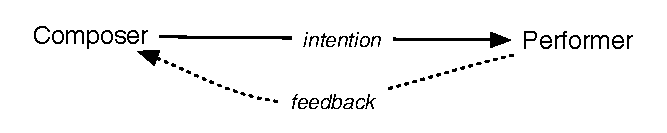
\includegraphics[width=0.5\columnwidth]{img/composer-performer}
  \caption{Intentionality in the documented session between Stefan and Love.}
  \label{cmp_perf}
 \end{center}
 \end{figure}

 \begin{figure}[!t]
  \begin{center}
   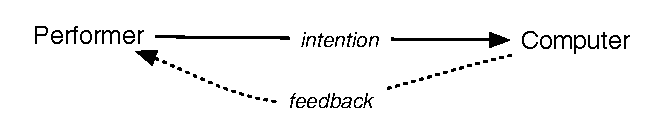
\includegraphics[width=0.5\columnwidth]{img/performer-computer}
   \caption{Intentionality at the performance in the suggested project. }
   \label{perf_cmp}
   \end{center}
 \end{figure}

Furthermore a few observations can be made that can be further
elaborated in the context of live electronic interactive music:
%. The
%observations can be summarized as:
 \begin{itemize}
  \item {Noise in communication is not a problem, it's an asset.

	We are used to think of a computer based interactive system as a
	cybernetic system in which information is transmitted from point
	A to point B and where great care is taken to avoid noise in the
	transmission. Think of the pedal that Stefan is using in Viken
	to step through the piece. If the signal going from the pedal to
	the Max/MSP patch running the piece was noisy or ambiguous it
	would probably be useless. `Almost a pressed pedal' is not a
	valid message in that system.
	
	In our joint project we will attempt to avoid the kind of binary
	oppositions that require a clean control signal path (such as
	the pressing of a pedal) in the design of the interactive
	system. It is our belief that this can be achieved in
	approaching the issues differently but more experiments has to
	be carried out. Obviously this will also affect the way the
	instrumental part is written.}

  \item {Direction is more important than synchronicity.

	A few remarks needs to be made regarding this if we want to
	successfully transfer this knowledge to a practical musical
	situation:
	\begin{itemize}
	 \item In the video Stefan and Love is not working in real
	       time. Time is not an issue - the result is not affected
	       if it takes them 15 years to finish the process. 
	 \item In a musical performance there's the musical time to pay
	       attention to which is an integral part of almost any
	       music.
	\end{itemize}
	Accordingly, the musical synchronization and low level time
	scale has to be dealt with; but on the structural level above
	that, perhaps a sensitive interactive real time performance
	system can deal more freely with time and distribute its events
	in relation to current and past input and that this approach
	will result in a more natural interaction from the point of view
	of the performer. In other words, we will argue for a dynamic
	score, a musical frame in which different paths can be taken,
	not so much on stylistic or esthetic grounds as because we
	believe it may result in an interesting interactive experience.

	Again, this is closely linked with how the music in general in
	composed.

	}
  \item {The initiative can shift independently of the esthesic and poietic
	processes.

	What this means in the context of an interactive real time
	performance system is that no matter what the current process is,
	and regardless of the current mode of interaction, the
	initiative can shift back and forth between the performer and
	the electronic part just as it does in the documented session
	between Stefan and Love..
	}
 \end{itemize}

The way the idea of the composer has been deconstructed in this study,
what remains of it is 'the one with the intention to create'(see figure
\ref{cmp_perf}). This is in accordance with Husserl's notion of
'intentionality' or Derrida's idea of 'la diff\'{e}rance'. This is not
to be confused with our term 'initiative' used in the graph. This
'intention' is, in the model we are imagining for our project,
transferred to the interpreter at the stage of performance. In other
words, the attributes we assign to the composer in the documented
session belongs to the interpreter at the stage of performance (see
figure \ref{perf_cmp}).


\begin{figure}[!ht]
\begin{center}
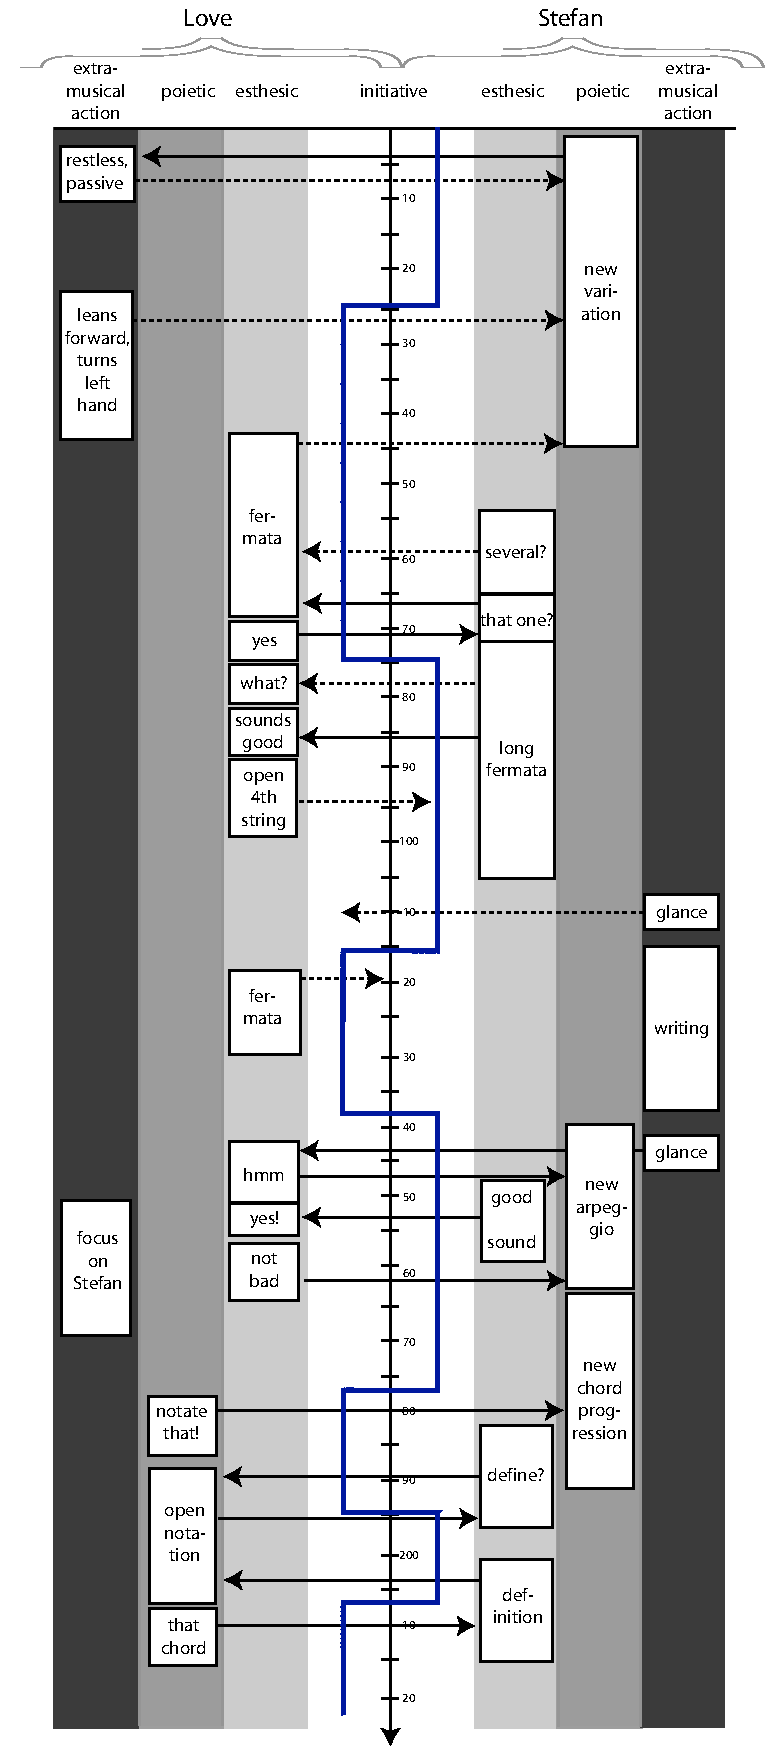
\includegraphics[width=0.8\columnwidth]{img/timeline_horiz}
\caption{A graph of the interaction between Stefan \"{O}stersj\"{o} and
 Love Mangs in the session analyzed in Section \ref{thevideo}. The scale
 in the center axis refers to line numbers in the transcription of the video.} \label{graph}
\end{center}
\end{figure}

%
%When building interactive systems noise is generally something we
%attempt at avoiding. 
%
%
%
%A more specific obstacle in the composition and implementation of an
%interactive piece of mixed media music is to collect and process
%relevant data that can be the object for the interaction. If we compare
%this issue with the situation in the analysis above there is a striking
%difference in the amount of information present \emph{on the surface} at the
%source.

\bibliography{bibliography}
\bibliographystyle{apalike}
\end{document}